\label{chapter:used-molecules}
The following molecules have been used to conduct experiments. Images show the molecules on a first layer copper crystal background (lattice constant \SI{2.55}{\angstrom}) to elucidate their size. Second and proceeding crystal layers are not shown for better visibility. All images show the molecules on the same substrate area (\SI{2.5}\times\SI{2.5}{\square\nm}). 

All the depicted molecules are modelled in Hyperchem\cite{_hyperchemtm_1111} and calculated for optimized geometry with the AM1+ method. Afterwards their positions are exported and remodelled in blender. Note that this does not change their geometry. It is only for better control of the output (faster and more accurate model building) and for some aesthetic reasons.

Unless stated otherwise the sample was kept at room temperature during dosage.

%%%%%%%%%%%%%%%%%%%%%%%%%%%%%%%%%%%%%%%%%%%%%%%%%%%%%%%%%%%%%%%%%%%%%%%%%%%%%%%%%%%%%%%%%%%
%%%%%%%%%%%%%%%%%%%%%%%%%%%%%%%%%%%nitro-prophines%%%%%%%%%%%%%%%%%%%%%%%%%%%%%%%%%%%%%%%%%
\paragraph{TBP}
\begin{itemize}
 \item Free base nitrophenyl - 5,10,15 Tri [di-[tert-butyl]-phenyl)] porphyrin \textbf{nitro porhin} \\ have 3(2) di-tert-butyl-phenyl groups attached to the macrocycle at the meso-positions of the molecule. The free meso-positions are occupied with nitrophenyl groups. If more than one functional group os prensent, one can destinguish between trans- and cis-configuration, whether the functional groups are opposite or neighbouring. See figure \ref{fig:nitro-trans-cis} for their graphical representation.
 \item In STM this molecules looks almost symmetrical, except the nitro-group which appears dark in STM, making the di-tert-butyl groups the most identifiable parts of the molecule.
 \item The appearence of STM data is correlated to the molecular configuration according to \cite{mishra_current-driven_2015} meaning that the lobes consiting of (3,5-di-tert-butylphenyl) are imaged as bright protrusions, while the functional nitro group is imaged fainter. This holds true for cis- and trans-substituted molecules.

\end{itemize}
Drawings for various functional groups and molecules can be found in \cite{jorgensen_salem_1973}

\begin{itemize}
\item[two-leg cis:] 	5,10-Bis(3,5-di-tert-butylphenyl)-15,20-Bis(Nitrophenyl)porphyrine
\item[two-leg trans:] 	5,15-Bis(3,5-di-tert-butylphenyl)-10,20-Bis(Nitrophenyl)porphyrine
\item[one-leg:] 	5,10,15-Tri(3,5-di-tert-butylphenyl)-20-(Nitrophenyl)porphyrine
\end{itemize}

\begin{figure}[ht]
 \begin{center}
 \subfigure[Single functional group]{
  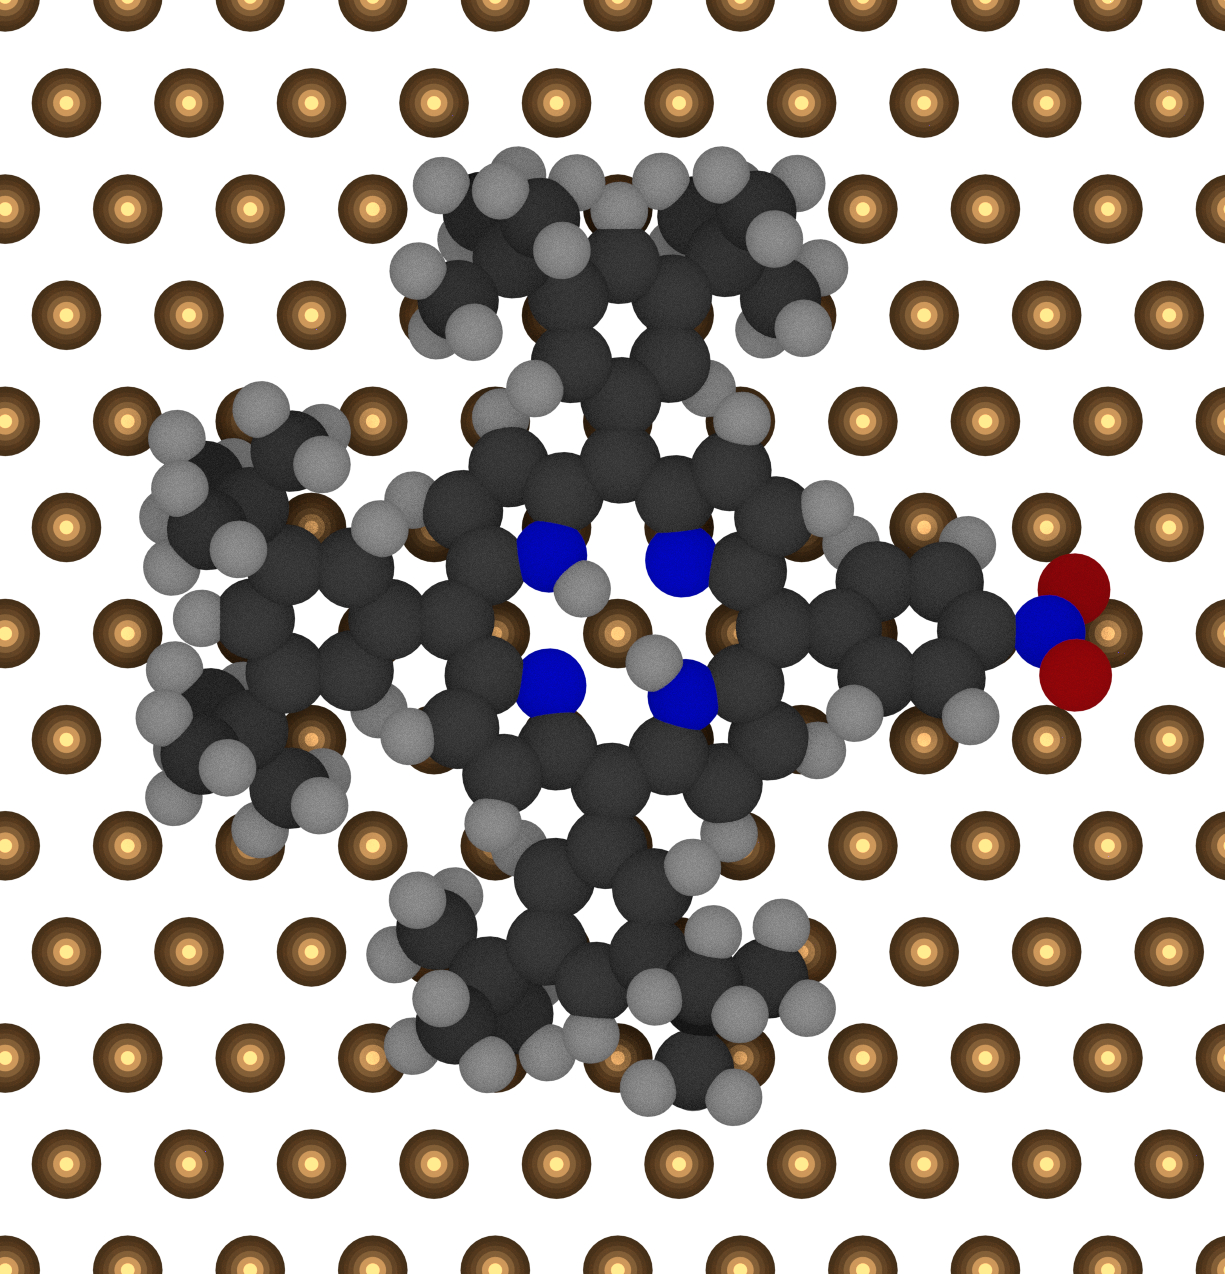
\includegraphics[width=0.3\textwidth]{./images/one-leg-TBP-top.jpg}
 }
 \subfigure[Trans-configuration]{
  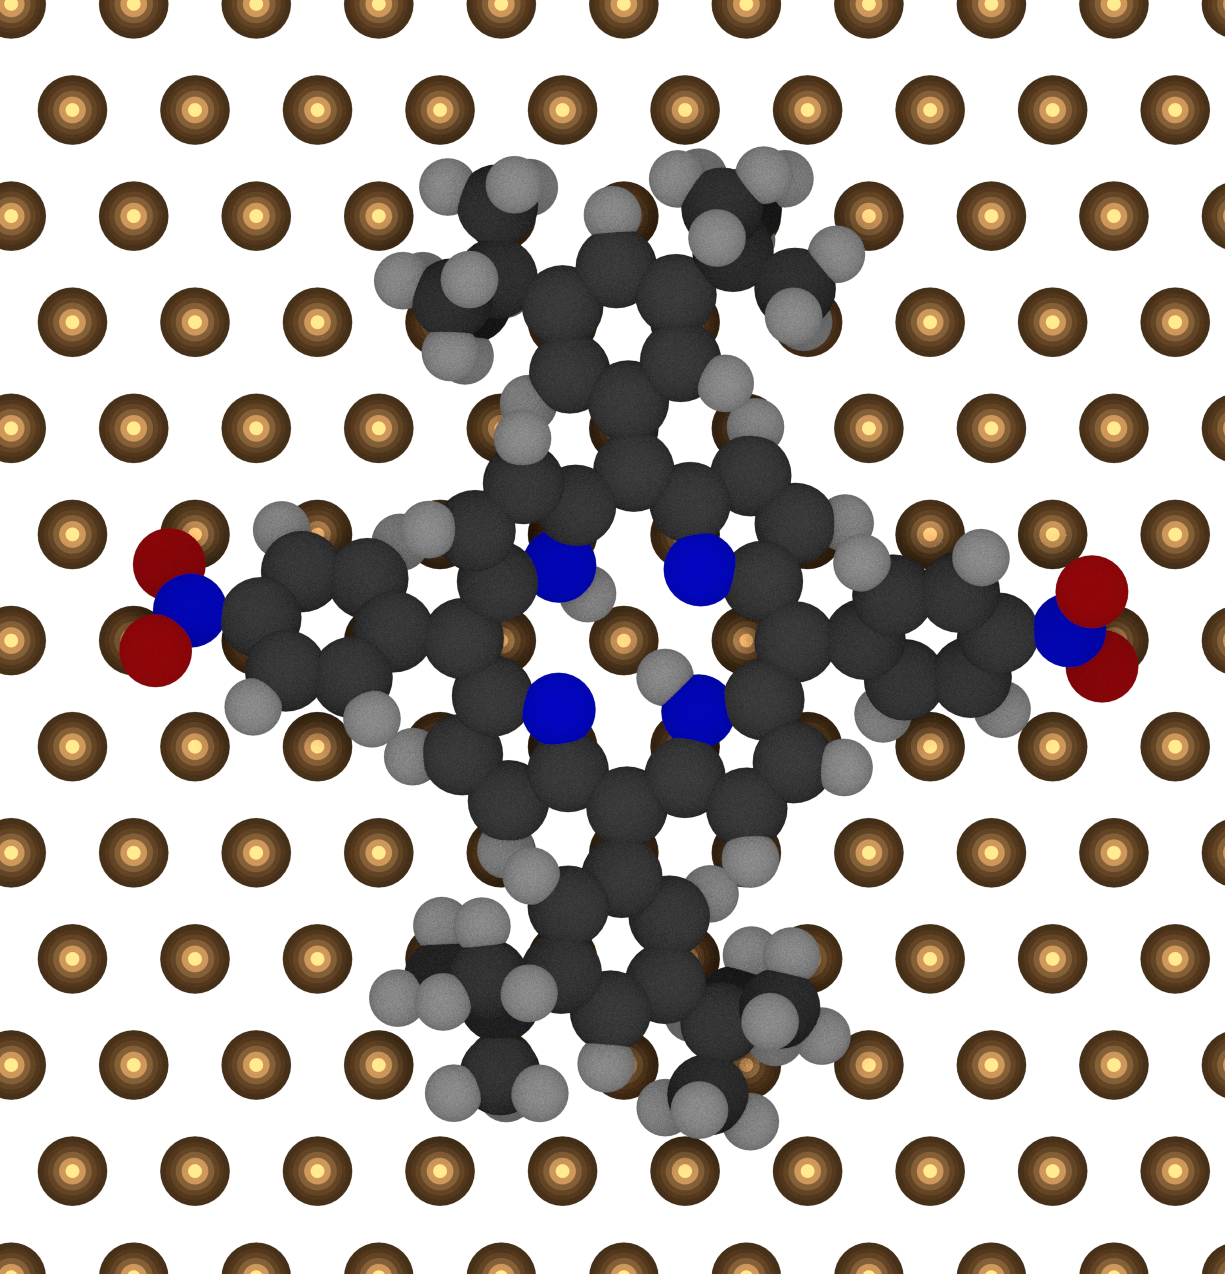
\includegraphics[width=0.3\textwidth]{./images/trans-TBP-top.jpg}
 }
 \subfigure[Cis-configuration]{
  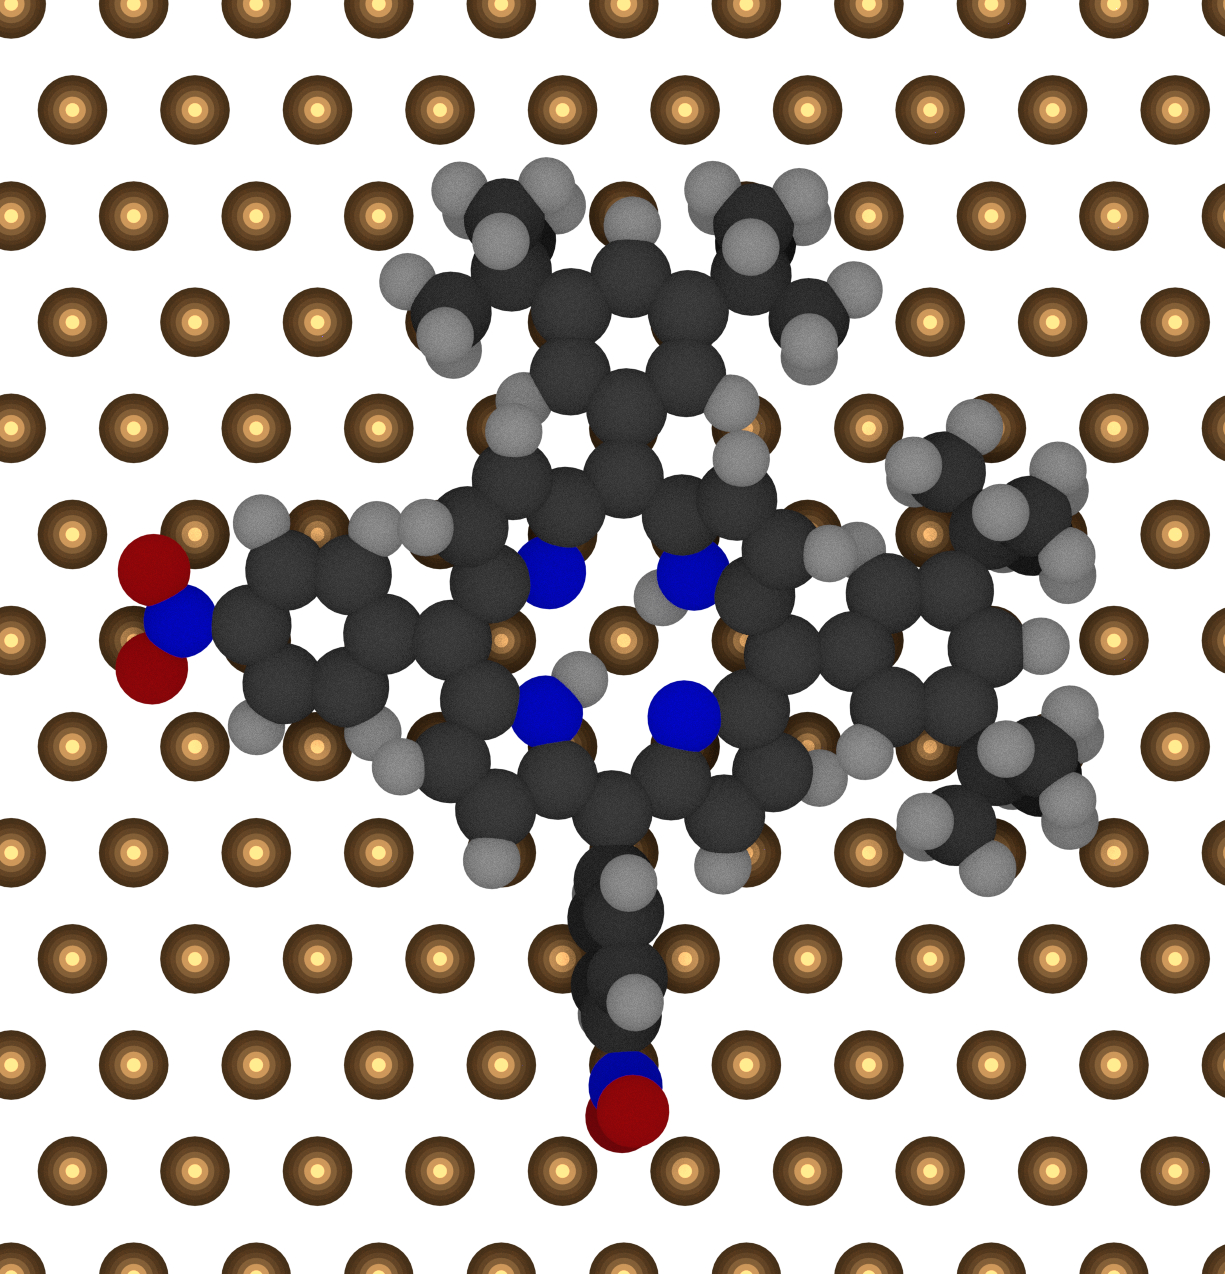
\includegraphics[width=0.3\textwidth]{./images/cis-TBP-top.jpg}
 }
 \end{center}
\caption{Functionalized tert-butyl-phenyl-porphines. Position of the functional nitrophenyl changes and determines its name.}
\label{fig:nitro-trans-cis}
\end{figure}
%%%%%%%%%%%%%%%%%%%%%%%%%%%%%%%%%%%%%%%%%%%%%%%%%%%%%%%%%%%%%%%%%%%%%%%%%%%%%%%%%%%%%%%%%%%
%%%%%%%%%%%%%%%%%%%%%%%%%%%%%%%%%%%	pyrenes   %%%%%%%%%%%%%%%%%%%%%%%%%%%%%%%%%%%%%%%%%
\paragraph{pyrenes}
\begin{itemize}
\item[cis-pyrene:] 1,8-Bis(4-Pyridylethynyl)pyrene
\item[trans-pyrene:] 1,6-Bis(4-Pyridylethynyl)pyrene
\item[tetra-pyrene:] 1,6,8,13-Tetra(4-Pyridylethynyl)pyrene
\end{itemize}

\begin{figure}[ht]
 \begin{center}
 \subfigure[Trans-configuration]{
  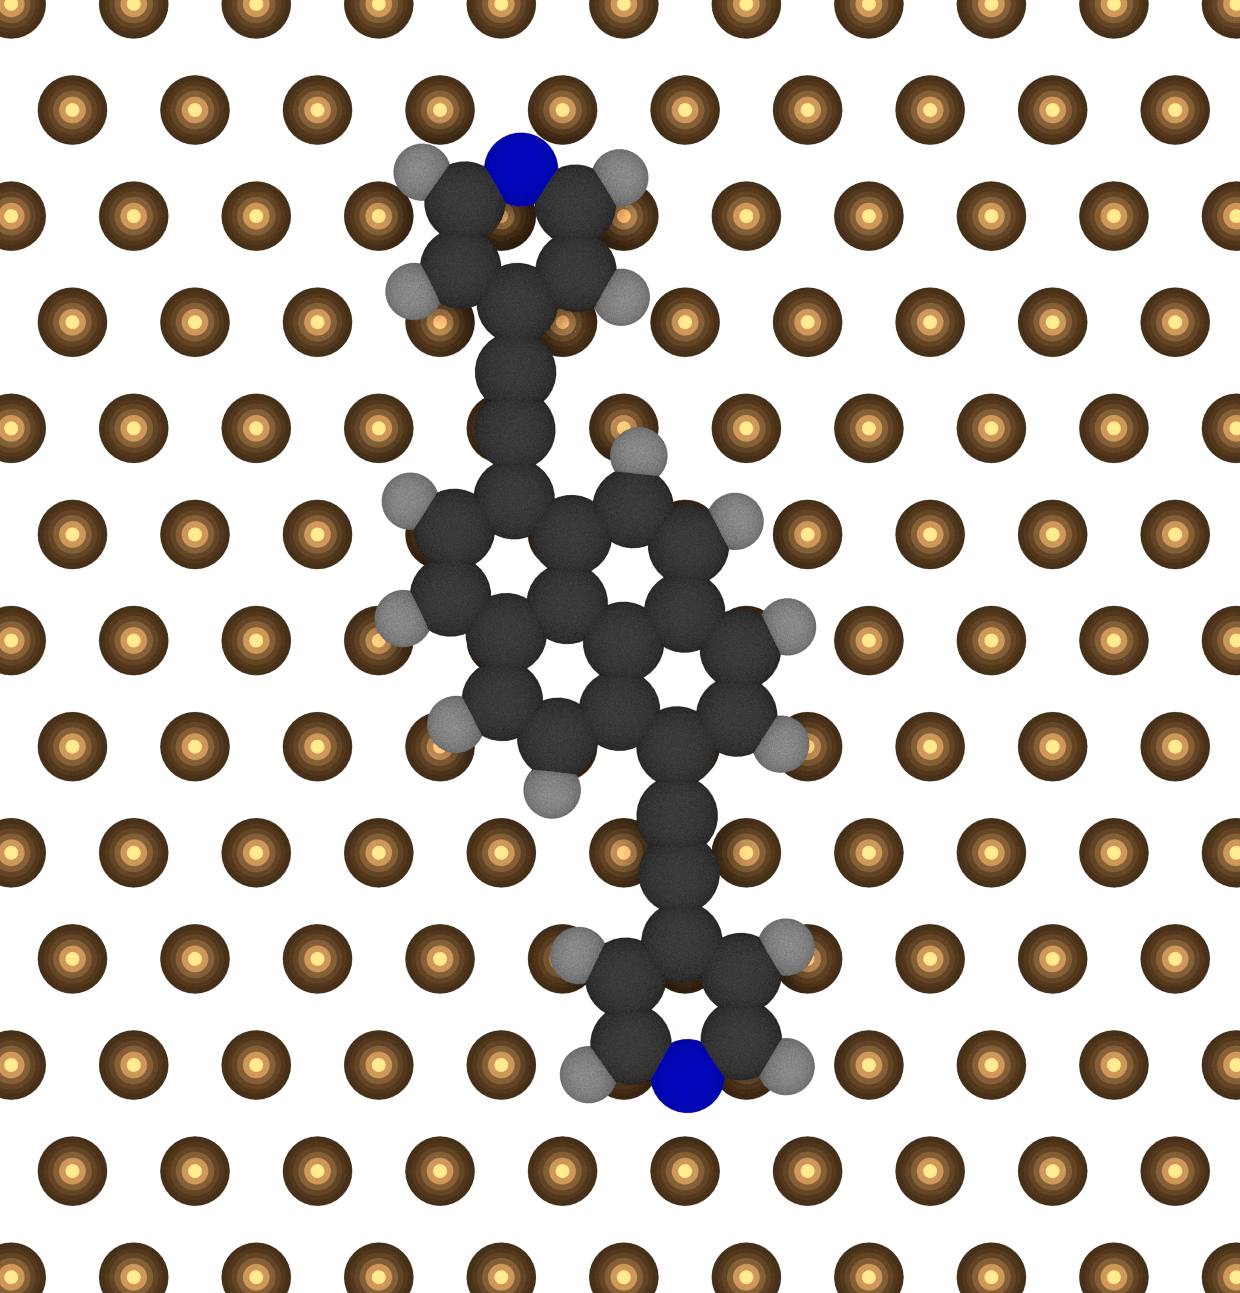
\includegraphics[width=0.3\textwidth]{./images/trans-pyrene-top.jpg}
 }
 \subfigure[Cis-configuration]{
  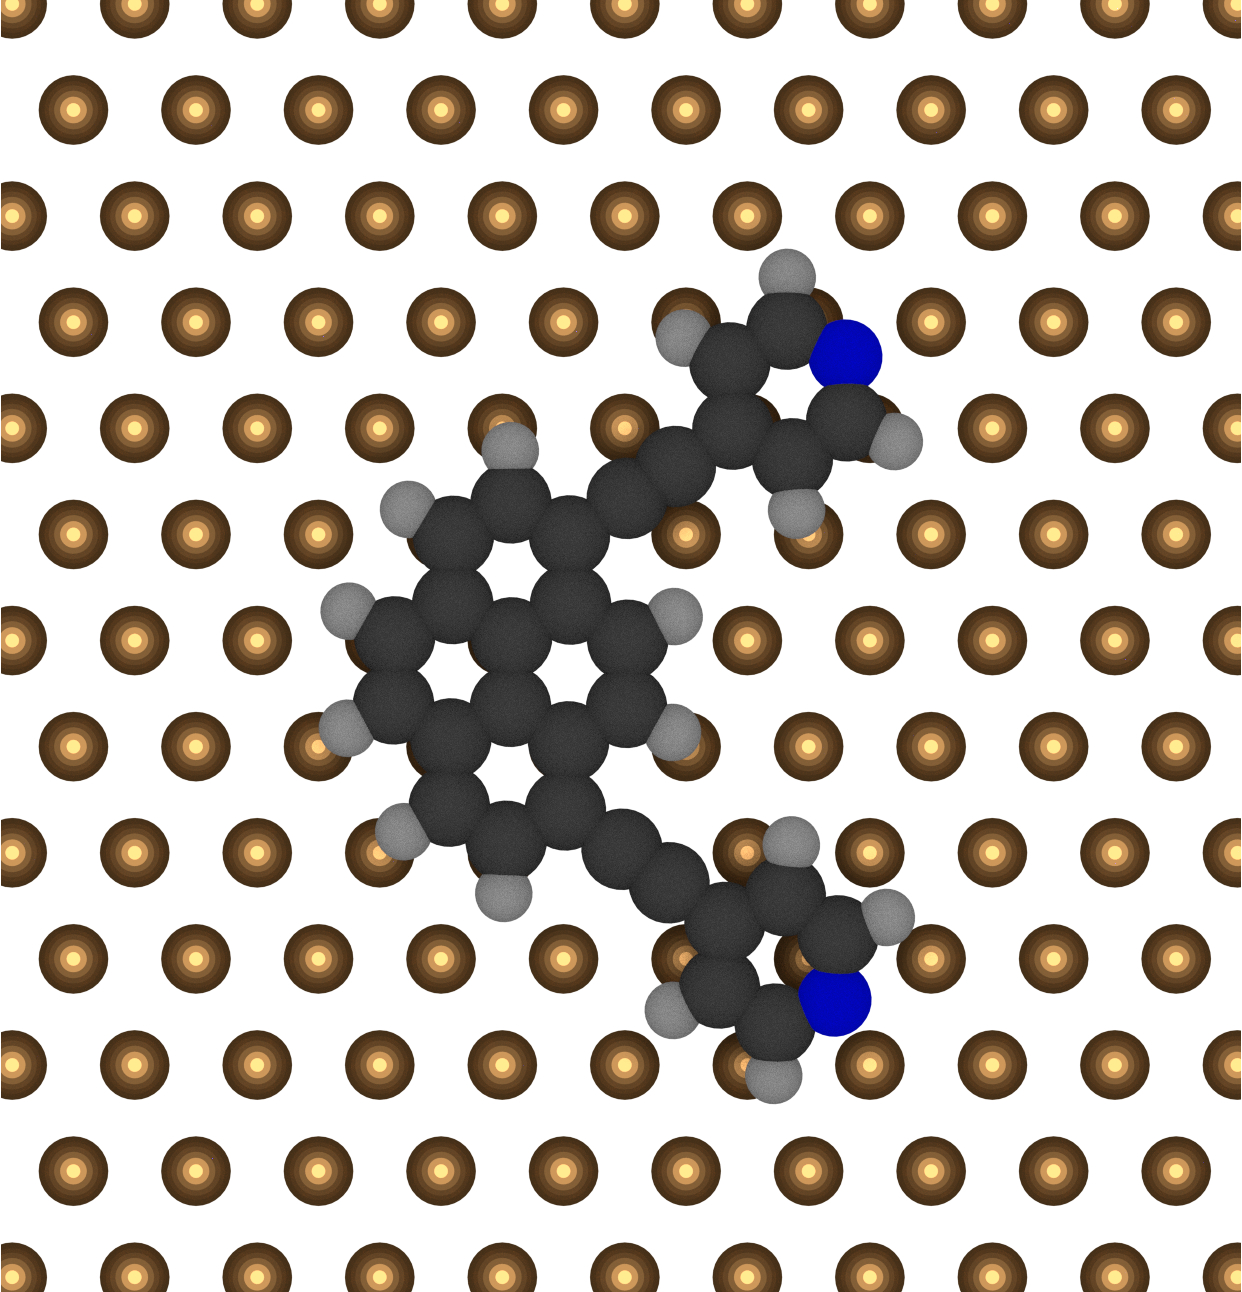
\includegraphics[width=0.3\textwidth]{./images/cis-pyrene-top.jpg}
 }
 \end{center}
\caption{Pyridyl-Pyrene molecules in trans- (a) and cis- (b) configuration}
\end{figure}
%%%%%%%%%%%%%%%%%%%%%%%%%%%%%%%%%%%%%%%%%%%%%%%%%%%%%%%%%%%%%%%%%%%%%%%%%%%%%%%%%%%%%%%%%%%
%%%%%%%%%%%%%%%%%%%%%%%%%%%%%%%%%%%	TPCN      %%%%%%%%%%%%%%%%%%%%%%%%%%%%%%%%%%%%%%%%%
\paragraph{TPCN}
TPCN can be evaporated with an OMBE. Temperatures used are typically \SI{490}{\celsius}, evaporation time depends on the intended coverage. 
\begin{itemize}
 \item [TPCN:] Tetra[(4-cyanophenyl)-phen-4-yl] porphyrin has four arms attached to the meso-positions of the macrocycle. Each is build up from two chained phenyl rings with one end attached to the macrocycle and the other one attached to a C-N end group.
\end{itemize}

\begin{figure}[ht]
 \begin{center}
  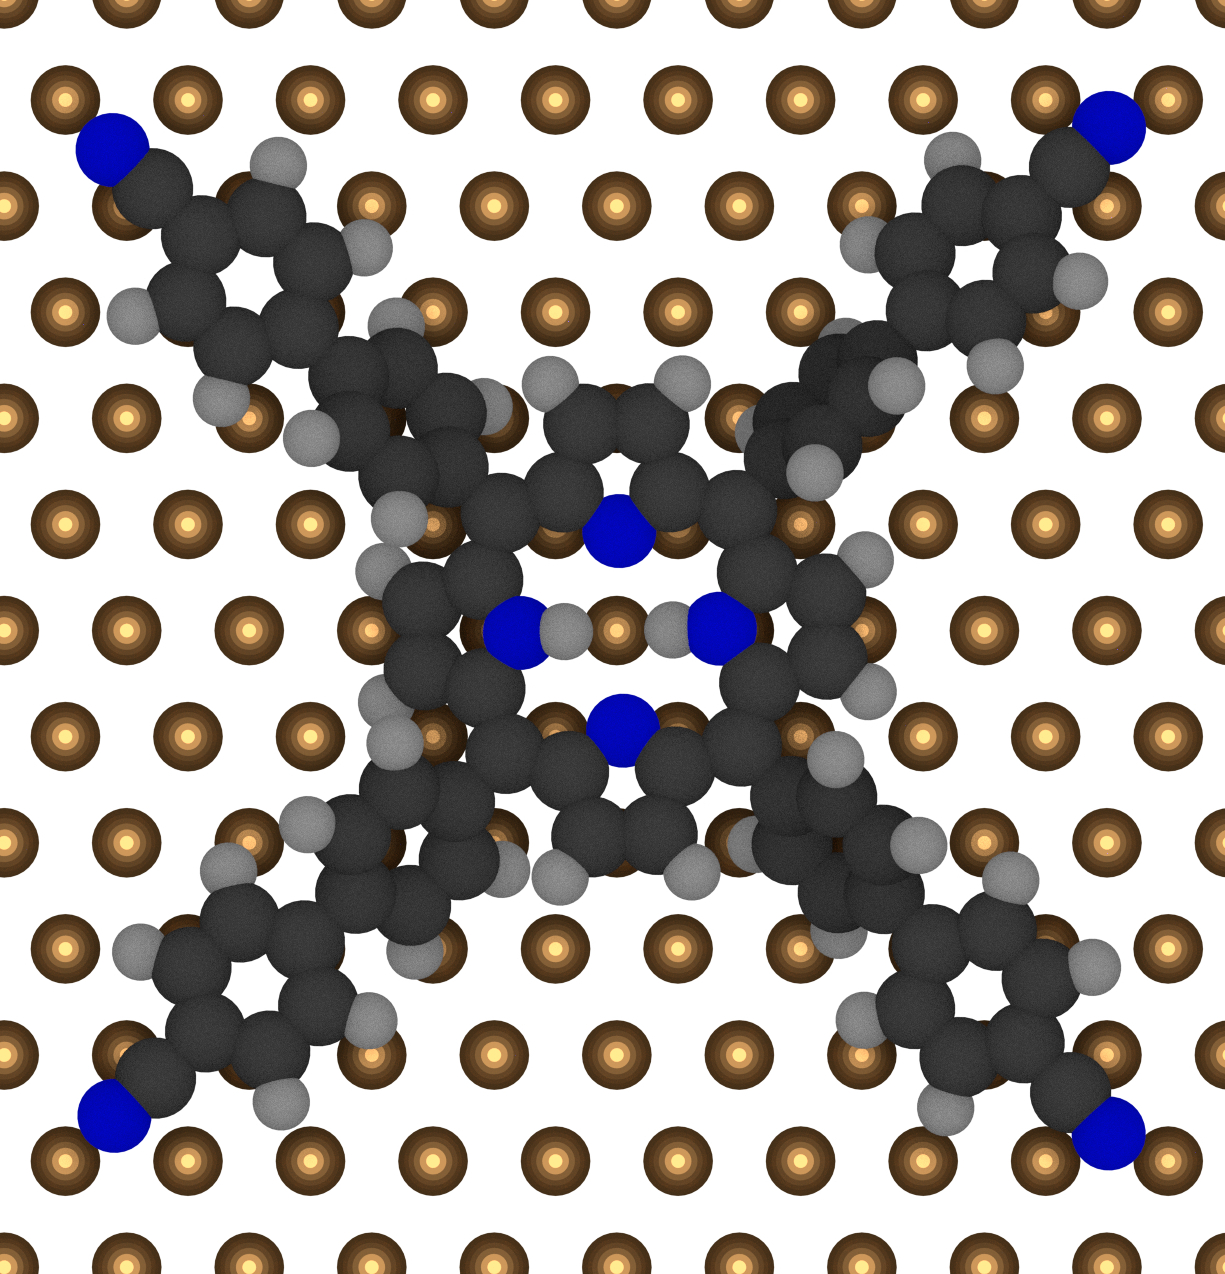
\includegraphics[width=0.3\textwidth]{./images/TPCN-top.jpg}
 \end{center}
\caption{TPCN}
\end{figure}
%%%%%%%%%%%%%%%%%%%%%%%%%%%%%%%%%%%%%%%%%%%%%%%%%%%%%%%%%%%%%%%%%%%%%%%%%%%%%%%%%%%%%%%%%%%
\begin{table}
 \centering
 \caption{Evaporation and degas temperatures used for different molecules.}
 \begin{tabular}{ccrc}
Name			& Configuration & Degas [\SI{}{\degreeCelsius}]	& Evaporate [\SI{}{\degreeCelsius}]	\\ \hline \hline 
TPCN			& ---		& ---		& 490		\\ \hline 
\multirow{3}{*}{TBP}	&single		& \SI{4}{\hour} @ \SI{200}{\degreeCelsius}& 390	\\
			&cis		& ---		& \SI{400}{\degreeCelsius}\\
			&trans		& \SI{4}{\hour} @ \SI{200}{\degreeCelsius} + \SI{1}{\hour} @ \SI{270}{\degreeCelsius}&\SI{370}{\degreeCelsius}\\ \hline 
\multirow{4}{*}{pyrene} & \multirow{3}{*}{cis}		& \SI{2}{\hour} @ \SI{180}{\degreeCelsius}&	\multirow{3}{*}{250}	\\
&&+ \SI{1}{\hour} @ \SI{200}{\degreeCelsius} + \SI{10}{\minute} @ \SI{235}{\degreeCelsius} 	&\\
&&+ \SI{1}{\hour} @ \SI{220}{\degreeCelsius}&\\ 
			&trans		& \SI{1}{\hour} @ \SI{230}{\degreeCelsius}		&\SI{265}{\degreeCelsius}		\\ \hline
\multirow{3}{*}{DCDB} & \multirow{3}{*}{---} & 1h @ \SIrange{100}{150}{\degreeCelsius}& \multirow{3}{*}{\SIrange{220}{240}{\degreeCelsius}}\\
&&+\SI{10}{\minute} @ \SI{170}{\degreeCelsius} + \SI{25}{\minute} @ \SI{200}{\degreeCelsius} & \\
&&+ \SI{40}{\minute} @ \SI{220}{\degreeCelsius}&\\
 \end{tabular}
\label{tab:molecule-temperatures}
\end{table}


%%%%%%%%%%%%%%%%%%%%%%%%%%%%%%%%%%%%%%%%%%%%%%%%%%%%%%%%%%%%%%%%%%%%%%%%%%%%%%%%%%%%%%%%%%%
%%%%%%%%%%%%%%%%%%%%%%%%%%%%%%%%%%%	helicenes %%%%%%%%%%%%%%%%%%%%%%%%%%%%%%%%%%%%%%%%%
\paragraph{helicenes}
\begin{itemize}
% \item[[7]-CN-helicene:] 2,16-Bis(cyano)-helicene
\item[Dicyano-Dibenzo-[5]helicene:] 7,8-Bis(cyano)-Dibenzo-helicene
\end{itemize}

% \begin{figure}[ht]
%  \centering
%  \subfigure[Top view]{
%   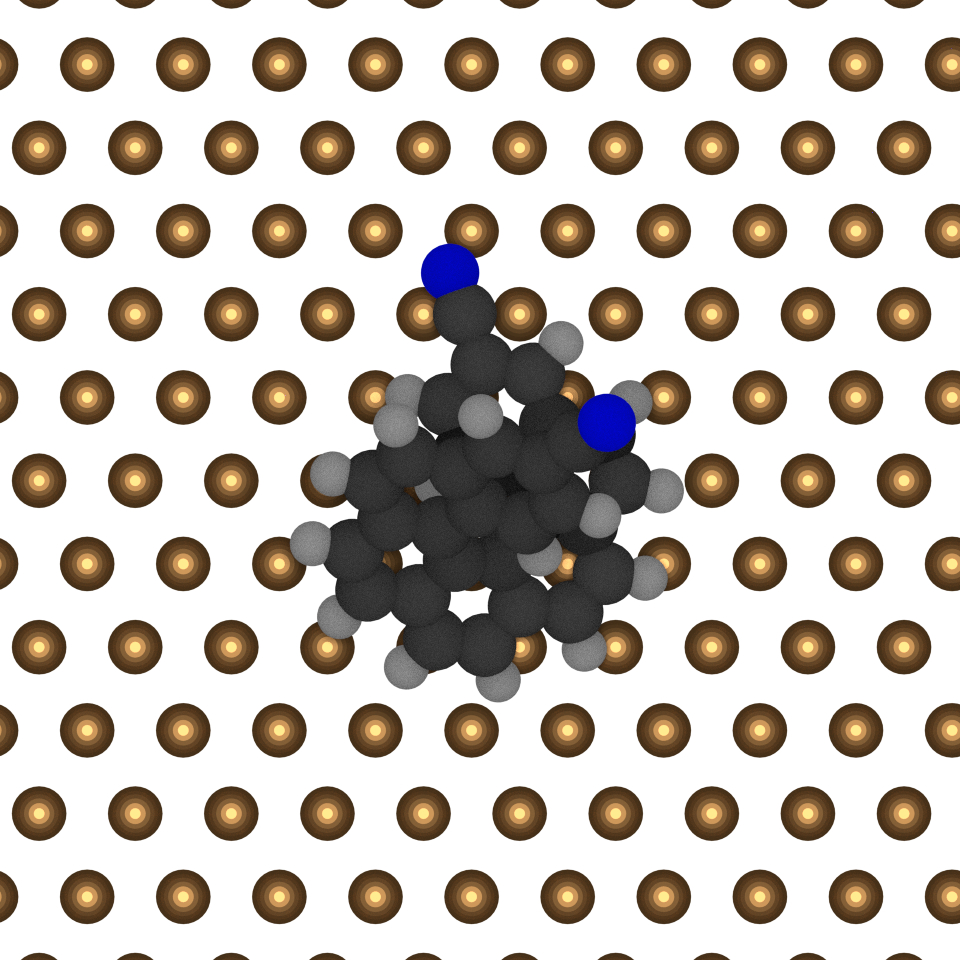
\includegraphics[width=0.3\textwidth]{./images/7-helicene-CN-AM1-top.jpg}
%   }
%  \subfigure[Sideview]{
%   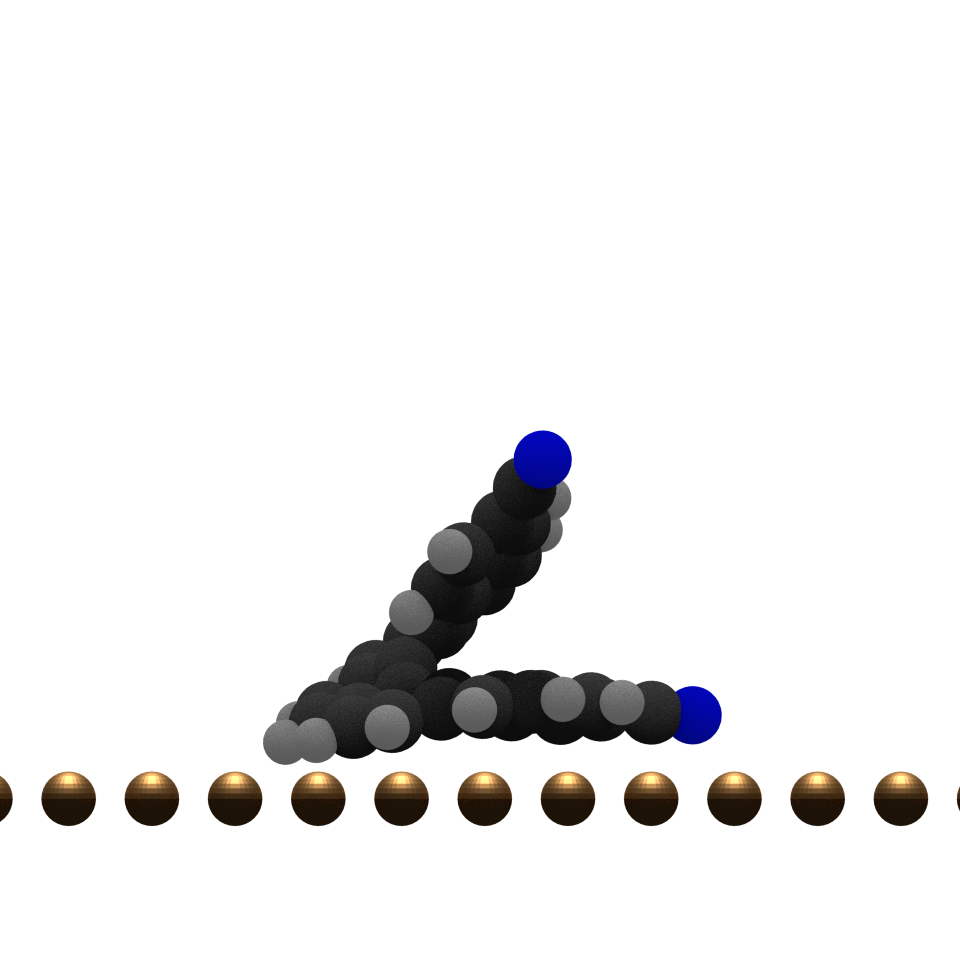
\includegraphics[width=0.3\textwidth]{./images/7-helicene-CN-AM1-side.jpg}
%   }
% \caption{[7]-CN-helicene on copper surface. a) Top view, b) side view}
% \end{figure}

\begin{figure}[ht]
 \centering
 \subfigure[Top view]{
  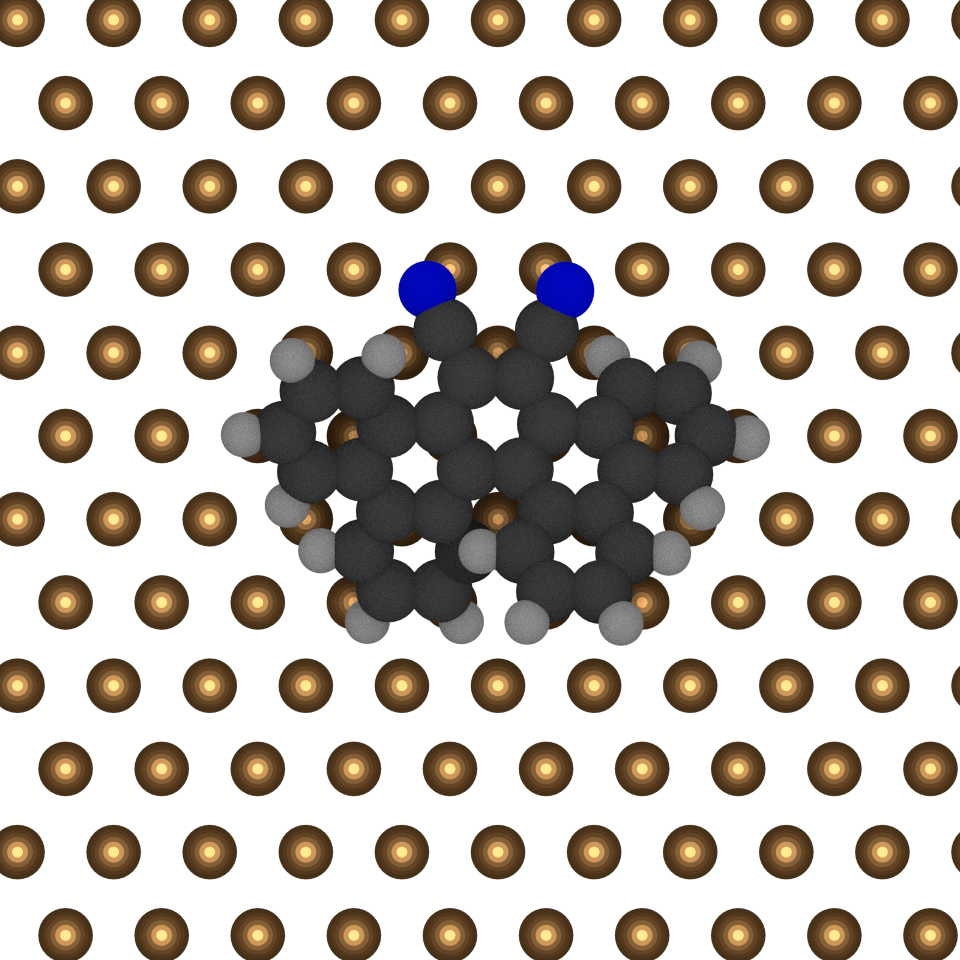
\includegraphics[width=0.3\textwidth]{./images/DCDB-AM1-top.png}
  }
 \subfigure[Sideview]{
  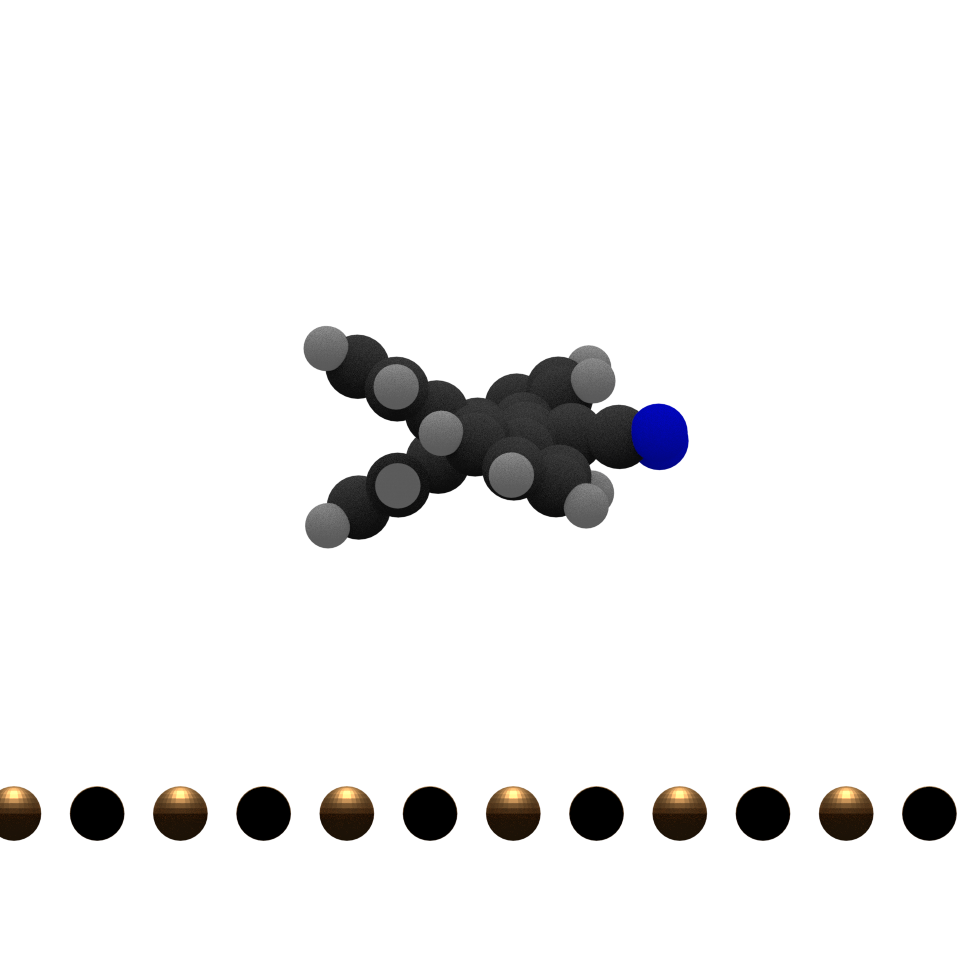
\includegraphics[width=0.3\textwidth]{./images/DCDB-AM1-side.png}
  }
\caption{DCDB on copper surface. a) Top view, b) side view}
\end{figure}

\paragraph{How to determine molecules' distance}
To determine the distance between molecules, one has to carefuly choose the points of interest. As a problem of STM imaging the contour of the molecules sometimes appears as more or less fuzzy shape. There is no sharp edge that one could take as start or end point of the profile. Therefore the center of the molecule is often used as reference point to measure the distance between two molecules (compare fig. \ref{fig:distance-molecules}). As the molecule has a square footprint, one can use the center in one direction (along profile 2/3) to determine the center in the other direction (profile 1). As one can see the three profiles match leading to a consistent center of the dimer. This is also shown as depression in profile 1. 

\begin{figure}[!ht]
\centering
\subfigure[Molecule with chosen profiles (1-3) indicated as white lines.]{
        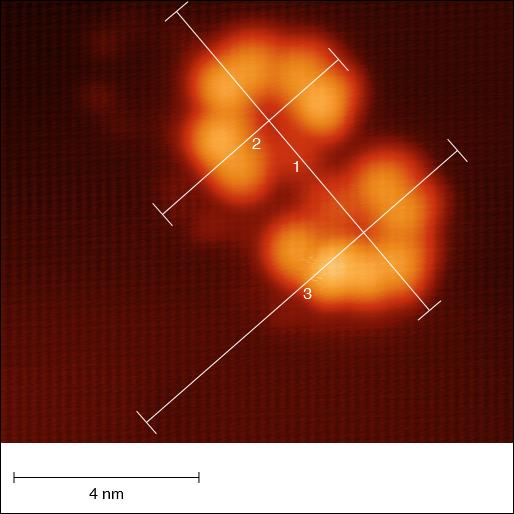
\includegraphics[width=0.45\textwidth]{./images/F150612-163956-dimer-loose.jpg}
}
\subfigure[Profiles 1-3 indicated in a).  Local minima in profile 2/3 indicate central positions in profile 1.]{
	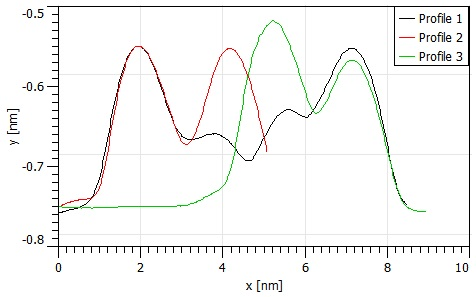
\includegraphics[width=0.45\textwidth]{./images/F150612-163956-profile-dimer-loose.jpg}
}
\caption{Sketch of how to determine the distance between two molecules. As the molecule is square (with the exception of one direction, one can determine the center of the molecule by comparing two 90 degree rotated profiles. Profile 1 goes through the symmetry axis, while profile 2 and 3 intersect profile 1 at the center. As the profile 2 and 3 look the same when starting at the buthyl groups, one can use the depression in profile 2 and 3 to determine the center of the molecule in profile 1.}
\label{fig:distance-molecules}
\end{figure}